\documentclass[onecolumn, letterpaper, 12pt]{report}

% insert any packages, environments, counters, etc here
\usepackage{graphicx}
\usepackage{hyperref}

\begin{document}
%insert document contents here

\section{Intro}

Conv Nets are a specialized kind of neural network for processing data that has a known, grid like topology. Examples include time series data, which can be thought of as a 1D grid takings samples at regular time intervals, and image data which can be thought of as a 2D grid of pixels. 

The name convolutional neural network implies that the network employs a mathematical operation called a \textbf{convolution}. CNNs use convolution in place of general matrix multiplication in at least one of their layers. 

\section{The Convolution Operation}

The convolution is an operation on two functions of a real valued argument. Suppose we are tracking the location of a spaceship with a laser sensor. The laser provides a single output $x(t)$
, the position of the space ship at time $t$. Both $x$ and $t$ are real valued. 

Now suppose our laser sensor is noisy. To obtain a less noisy estimate of the ships position, we would like to average together several measurements. More recent measurements are more relevant, so we will want to give a weighted average with more weight to recent measurements. We can do this by applying a weighting function $w(a)$ where $a$ is the age of the measurement. 

If we apply such a weighted average operation at every moment, we obtain a new function $s$ providing a smoothed estimate of the position of the spaceship 

\begin{center}
  $s(t) = \int x(a) w(t - a) da$
\end{center}

This operation is called a convolution and is typically denoted with an asterisk

\begin{center}
  $s(t) = (x * w)(t) $
\end{center}


In our example, $w$ needs to be a valid probability distribution. In convolutional network terminology, the first argument ($x$) to the convolution is often referred to as the \textbf{input} and the second argument ($w$) is known as the \textbf{kernel}. The output is sometimes referred to as the \textbf{feature map}.

For a discrete convolution, we can assume that $t \in N$
. Then we can define the discrete convolution as 


\begin{center}
  $s(t) = (x * w)(t) = \sum\limits_{a = -\infty}^{\infty} x(a)w(t - a)$
\end{center}

In ml applications, the input is generally a multidimensional array of data and the kernel is usually a multidimensional array of parameters that are adapted by the learning algorithm. 

We often use convolutions over more than one axis at a time. For example, if we use a two dimensional image $I$ as our input, we also want to use a two dimensional kernel $K$: 

\begin{center}
  $s(i, j) = (I * K)(i, j) = \sum\limits_m \sum\limits_nI(m,n) K(i-m, j-n)$
\end{center}

Convolution is commutative, so equivalently we could write 

\begin{center}
  $s(i, j) = (I * K)(i, j) = \sum\limits_m \sum\limits_nI(i-m,j-n) K(m, n)$  
\end{center}

While the commutativity of convolutions is useful for writing proofs, in practice neural network libraries often implement a related function called \textbf{cross-correlation}, which is the same as convolution but without flipping the kernel: 

\begin{center}
  $s(i, j) = (I * K)(i, j) = \sum\limits_m \sum\limits_nI(i+m,j+n) K(m, n)$
\end{center}

Discrete convolution can be viewed as multiplication by a matrix. The matrix has several entries constrained to be equal to other entries. For example, for univariate discrete convolution, each row of the matrix is constrained to be equal to the row above shifted by one element. This is known as a \textbf{Toeplitz matrix}. In two dimensions, a \textbf{doubly block circulant matrix} corresponds to convolution. 

In addition to these constraints, convolution usually cooresponds to a very sparse matrix. This is because the kernel is usually much smaller than the input image. Any neural network algorithm that works with matrix multiplication and does not depend on specific properties of the matrix structure should work with convolution without requiring further changes to the network. 

\begin{figure}[h]
  \centering
  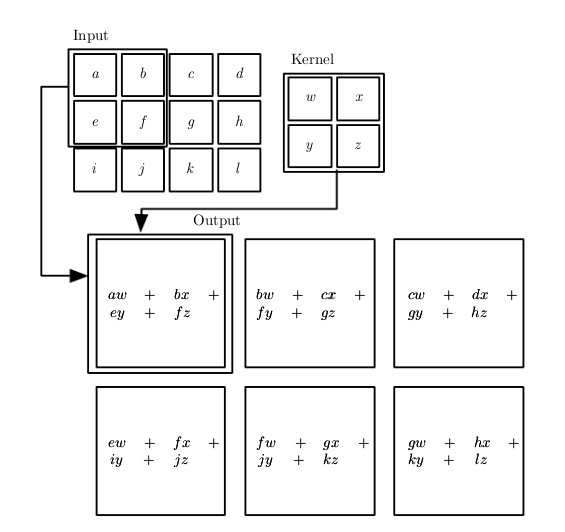
\includegraphics[width=0.7\textwidth]{conv_2d.png}
  \caption{2-D convolution without kernel flipping}
\end{figure}

\section{Motivation}

Convolution leverages three important ideas that can help improve a machine learning system: 

\begin{enumerate}
\item sparse interactions
\item parameter sharing
\item equivariant representations
\end{enumerate}

\subsection{sparse interactions}

Traditional neural networks layers use matrix multiplication by a matrix of parameters with a separate parameter describing the interaction between each input unit and each output unit. This means that each input unit interacts with each output unit.

Convolutional neural networks in contrast typically have \textbf{sparse interactions} (also referred to as sparse connectivity or sparse weights). This is accomplished by making the kernel smaller than the input. When processing an image, there may be thousands or millions of pixels, but we can detect small meaningful features such as edges with kernels that only occupy tens of pixels. This means we can store fewer parameters, reducing the space and time requirements and improving statistical efficiency. 

\begin{figure}[h]
  \centering
  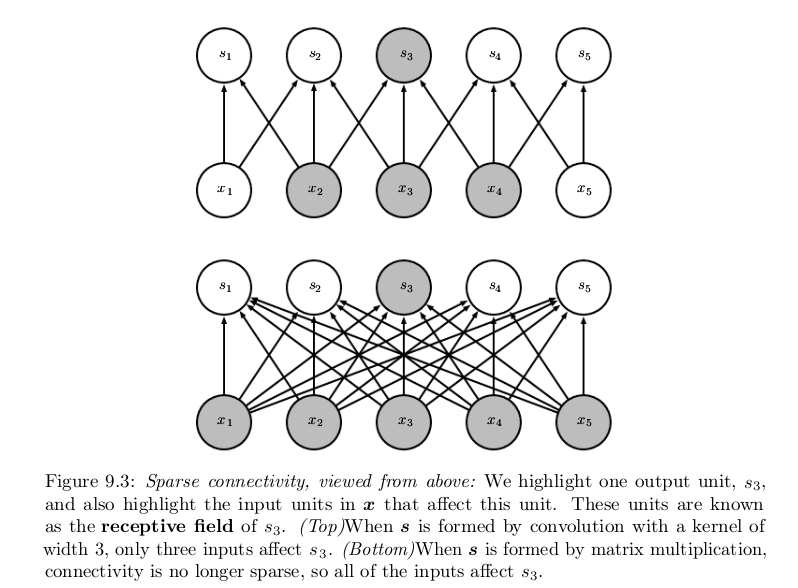
\includegraphics[width=0.7\textwidth]{sparse_connectivity.png}
\end{figure}

\subsection{parameter sharing}

\textbf{Parameter sharing} refers to using the same parameter for more than one function in a model. In a traditional network, we have \textbf{tied weights}. This means that the value of a weight applied to one input is tied to the value of a weight applied elsewhere. 

In a conv net, each member of the kernel is used at every position of the input (except perhaps the boundary pixels, depending on the design decisions). The parameter sharing used by the convolution operation means that rather than learning a separate set of parameters for every location, we can learn only one set. Convolution is thus dramatically more efficient than dense matrix multiplicationin terms of the memory requirements and statistical efficiency. 

\begin{figure}[h]
  \centering
  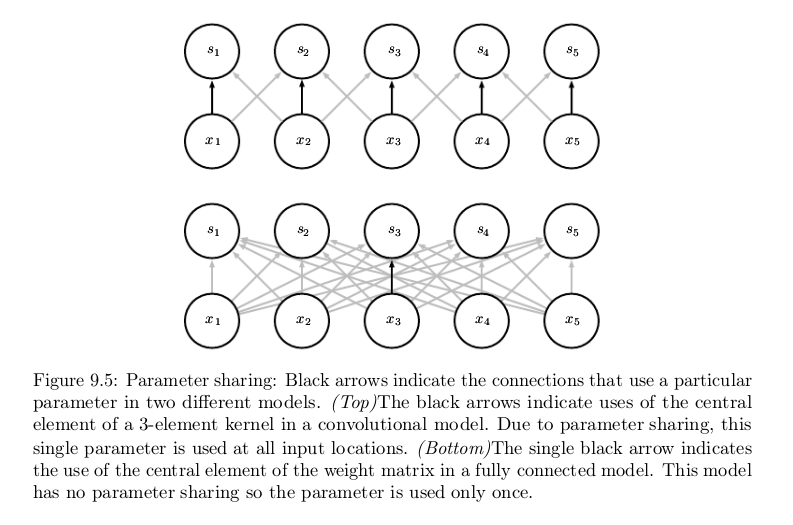
\includegraphics[width=0.7\textwidth]{param_sharing.png}
\end{figure}

\subsection{equivariance}

In the case of convolution, the particular form of parameter sharing causes the layer to have a property called \textbf{equivariance} to translation. To say a function is equivariant means that if the input changes, the output changes in the same way. Specifically, a function $f(x)$ is equivariant to a function $g$ if $f(g(x)) = g(f(x))$. In the case of convolution, if we let $g$ be any function that translates the input, i.e. shifts it, then the convolution function is equivariant to $g$. 

Convolution is not naturally equivariant to some other transformations, such as changes in the scale or rotation of an image. Other mechanisms are necessary for handling these kinds of transformations. 

\section{Pooling}

A typical layer of a convolutional neural network consists of three stages: 

1. The layer performs several convolutions in parallel to produce a set of linear activations.
2. Each linear activation is run through a nonlinear activation function, such as ReLU
3. This stage is sometimes called the \textbf{detector} stage. We use a \textbf{pooling function} to modify the output of the layer further. 

A pooling function replaces the output of the net at a certain location with a summary statistic of the nearby outputs. For example, max pooling returns the maximum output within a rectangular neighborhood. Other popular pooling functions include the average, the $L^2$ norm, or a weighted average based on the distance from the central pixel. 

\begin{figure}[h]
  \centering
  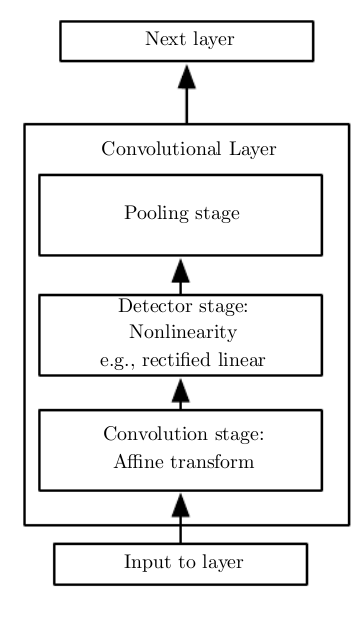
\includegraphics[width=0.3\textwidth]{conv_layer.png}
\end{figure}

In all cases, pooling helps to make the representation become approximately invariant to small translations of the input. Invariance to local translation can be a very useful property if we care more about whether some feature is present than exactly where it is. The use of pooling can be viewed as adding an infinitely strong prior that the function the layer learns must be invariant to small translations. When this assumption is correct, it can greatly improve the efficiency of the network. 

For many tasks, pooling is essential for handling inputs of varying size. For example, if we want to classify images of variable size, the input to the classification layer must have a fixed size. This is usually accomplished by varying the size of an offset between pooling regions so that the classification layer always receives the same number of summary statistics regardless of the input size. 

Some theoretical work gives guidance on which kinds of pooling to use in various situations (Boureau et al, 2010):

\begin{quote}
\href{https://www.di.ens.fr/willow/pdfs/icml2010b.pdf}{A Theoretical Analysis of Feature Pooling in Visual Recognition}  
\end{quote}

\begin{quote}
  Many modern visual recognition algorithms incorporate a step of
  spatial ‘pooling’, where the outputs of several nearby feature
  detectors are combined into a local or global ‘bag of features’, in
  a way that preserves task-related information while removing
  irrelevant details. Pooling is used to achieve invariance to image
  transformations, more compact representations, and better robustness
  to noise and clutter. Several papers have shown that the details of
  the pooling operation can greatly influence the performance, but
  studies have so far been purely empirical. In this paper, we show
  that the reasons underlying the performance of various pooling
  methods are obscured by several confounding factors, such as the
  link between the sample cardinality in a spatial pool and the
  resolution at which low-level features have been extracted. We
  provide a detailed theoretical analysis of max pooling and average
  pooling, and give extensive empirical comparisons for object
  recognition tasks.
\end{quote}

It is also possible to dynamically pool features together, for example, by running a clustering algorithm on the locations of interesting features (Boureau et al, 2011). This approach yields a different set of pooling regions for each image. 

\begin{quote}
\href{https://www.di.ens.fr/~fbach/boureau-iccv-11.pdf}{Ask the locals: multi-way local pooling for image recognition}
\end{quote}

\begin{quote}
  Invariant representations in object recognition systems are
  generally obtained by pooling feature vectors over spatially local
  neighborhoods. But pooling is not local in the feature vector space,
  so that widely dissimilar features may be pooled together if they
  are in nearby locations. Recent approaches rely on sophisticated
  encoding methods and more specialized codebooks (or dictionaries),
  e.g., learned on subsets of descriptors which are close in feature
  space, to circumvent this problem. In this work, we argue that a
  common trait found in much recent work in image recognition or
  retrieval is that it leverages locality in feature space on top of
  purely spatial locality. We propose to apply this idea in its
  simplest form to an object recognition system based on the spatial
  pyramid framework, to increase the performance of small dictionaries
  with very little added engineering. Stateof-the-art results on
  several object recognition benchmarks show the promise of this
  approach.
\end{quote}

Another approach is to learn a single pooling structure that is then applied to all images (Jia et al, 2012)

\begin{quote}
  \href{http://www.icsi.berkeley.edu/pubs/vision/beyondspatial12.pdf}{Beyond Spartial Pyramids: Receptive Field Learning for Pooled Image Features}
\end{quote}

\begin{quote}
  In this paper we examine the effect of receptive field designs on
  classification accuracy in the commonly adopted pipeline of image
  classification. While existing algorithms usually use manually
  defined spatial regions for pooling, we show that learning more
  adaptive receptive fields increases performance even with a
  significantly smaller codebook size at the coding layer. To learn
  the optimal pooling parameters, we adopt the idea of
  over-completeness by starting with a large number of receptive field
  candidates, and train a classifier with structured sparsity to only
  use a sparse subset of all the features. An efficient algorithm
  based on incremental feature selection and retraining is proposed
  for fast learning. With this method, we achieve the best published
  performance on the CIFAR-10 dataset, using a much lower dimensional
  feature space than previous methods.
\end{quote}

\section{Convolution and Pooling as an Infinitely Strong Prior}

Priors can be considered weak or strong depending on how concentrated the probability density in the prior is. A weak prior is a distribution with high entropy, such as a Gaussian with high variance. Such a prior allows the data to move the parameters more or less freely. A strong prior has very low entropy, such as a Gaussian with low variance. Such a prior plays an active role in determining where the parameters end up. An infinitely strong prior places zero probability on some parameters and says that these prarameter values are completely forbidden, regardless of any support from the data. 

We can imagine a convolutional net as being similar to a fully connected net, but with an infinitely strong prior over its weights. This infinitely strong prior says that the weights for one hidden unit must be identical to the weights of its neighbor, but shifted in space. This says that the function the layer should learn contains only local interactions and is equivariant to small translations. 

Implementing a fully connected convnet would be ridiculously wasteful, but considering a convolution as an infinitely strong prior can give us insight into how convolutional networks work. A prior is only useful when the assumptions made by the prior are reasonably accurate. If a task relies on preserving the precise spatial information, then using pooling on all features can increase the training error. When a task involves incorporating information from very distant locations in the input, then the prior imposed by convolution may be inappropriate. 

Some convolutional network architectures (Szegedy et al, 2014) are designed to use pooling on some channels, but not on other channels in order to get highly invariant features and features that will not underfit when the translation invariance prior in incorrect. 

\begin{quote}
\href{https://arxiv.org/pdf/1409.4842.pdf}{Going Deeper with Convolutions}  
\end{quote}

\begin{quote}
  We propose a deep convolutional neural network architecture
  codenamed Inception, which was responsible for setting the new state
  of the art for classification and detection in the ImageNet
  Large-Scale Visual Recognition Challenge 2014 (ILSVRC14). The main
  hallmark of this architecture is the improved utilization of the
  computing resources inside the network. This was achieved by a
  carefully crafted design that allows for increasing the depth and
  width of the network while keeping the computational budget
  constant. To optimize quality, the architectural decisions were
  based on the Hebbian principle and the intuition of multi-scale
  processing. One particular incarnation used in our submission for
  ILSVRC14 is called GoogLeNet, a 22 layers deep network, the quality
  of which is assessed in the context of classification and detection.
\end{quote}

\section{Variants of the Basic Convolution Function}

Assume we have a 4D kernel tensor $K$ with element $K_{i, j, k, l}$ giving the connection strength between a unit in channel i of the output and a unit in channel j of the input, with an offset of k rows and l columns between the output unit and the input unit. Assume our input consists of observed data $V$ with element $V_{i,j,k}$ giving the value of the input unit within channel i at row j and column k. Assume our output consists of $Z$ with the same format as $V$. If $Z$ is produced by convolving $K$ across $V$ without flipping $K$, then 

\begin{center}
  $Z_{i, j, k} = \sum\limits_{l,m,n} V_{l, j+m-1}K_{i,l,m,n}$
\end{center}

We may wish to skip over some of the positions of the kernel in order to reduce the computational cost (at expense). We can think of this as downsampling the output of the full convolution function. If we wish to sample only every $s$ pixels in each direction in the output, then we can define a downsampled convolution function c such that 

\begin{center}
  $Z_{i, j, k} = c(K, V, s)_{i, j, k} = \sum\limits_{l, m, n}[V_{l, (j-1) \times s + m, (k-1) \times s+n}K_{i, l, m, n}]$
\end{center}

We refer to $s$ as the \textbf{stride} of the downsampled convolution. It is also possible to define a separate stride for each direction of motion. 

One essential feature of any convolutional network is its ability to implicitly zero pad the input V in order to make it wider. Without this, the width of the representation would shrink with each layer. Without padding we would need to choose between shrinking the spatial extent of the network rapidly and using small kernels, both of which limit the expressive power of the network. 

Three special cases of zero-padding settings are worth mentioning :


\begin{enumerate}

\item No zero-padding whatsoever. This is called the \textbf{valid} convolution. In it the convolutional kernel is only allowed to visit positions where the entire kernel is contained entirely within the image. 

\item Just enough zero-padding to keep the size of the output equal to the size of the input. This is called the \textbf{same} convolution. Since the operation of convolution doesn't change the size of the input, these can handle as many layers as the hardware can. However, the input pixels near the border influence fewer output pixels than the input pixels near the center. This can make the border pixels somewhat underrepresented in the model. 

\item Enough zeroes are added for every pixel to be visited k times in each direction, resulting in an output image of width $m + k + 1$. This is called the \textbf{full} convolution. In this case, the output pixels near the border are a function of fewer pixels than the outputs near the center. This makes it difficult to learn a single kernel that performs well at all positions in the convolutional feature map. 

\end{enumerate}


Usually the optimal amount of zero-padding lies somewhere between valid and same convolution. 

\begin{figure}[h]
  \centering
  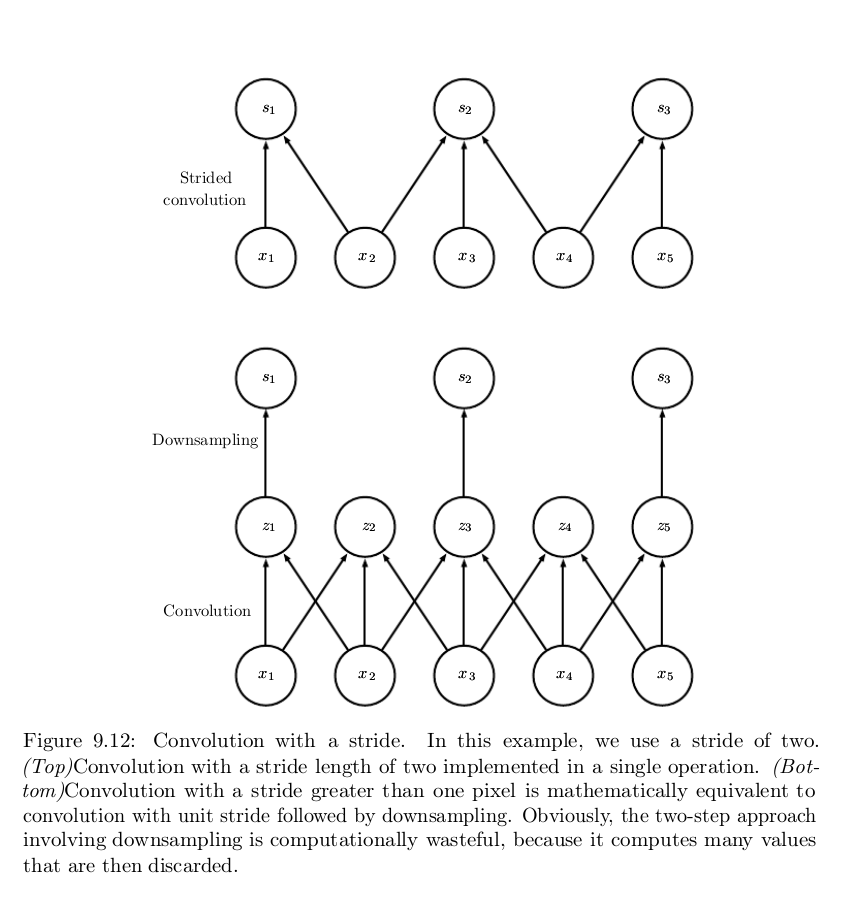
\includegraphics[width=0.7\textwidth]{strides.png}
\end{figure}

In some cases, we do not actually want to use convolution, but rather locally connected layers (LeCun, 1986, 1989). In this case, the adjacency matrix in the graph of our MLP is the same, but every connection has its own weight, specified by a 6D tensor $W$. The indices into $W$ are, respectively: i, the output channel, j, the output row, k, the output column, l, the input channel, m, the row offset within the input, and n, the column offset within the input. 

The linear part of a locally connected layer is then given by 

\begin{center}
  $Z_{i, j, k} = \sum\limits_{l, m, n}[V_{l,j+m-1,k+n-1w_{i,j,k,l,m,n}}]$
\end{center}

This is sometimes also called \textbf{unshared convolution}, because it is a similar operation to discrete covolution with a small kernel, but without sharing parameters across locations. 

\textbf{I had a bunch of notes for the rest of the section, but my computer froze and didn't save anything. Read from 350 - 358 for the information.}

\section{Structured Outputs}

Convolutional networks can be used to output a high dimensional, structured object, rather than just predicting a class label for a classification task or a real value for a regression task. Typically this object is just a tensor, emitted by a standard convolutional layer. 

For example, the model might emit a tensor $S$ where $S_{i,j,k}$ is the probability that pixel $(j,k)$ of the input to the network belongs to class $i$. This allows the model to label every pixel in an image and draw precise masks that follow the outlines of individual objects. 

One strategy for pixelwise labeling of images is to produce an initial guess of the image labels, then refine the initial guess using the interactions between neighboring pixels. Repeating this refinement step several times corresponds to using the same convolutions at each stage, sharing weights between the last layers of the deep net. This makes the sequence of computations performed by the successive convolutional layers with weights shared across layers a particular kind of recurrent network. 

Once the prediction for each pixel is made, we can use other methods to segment the image into regions. The general idea is that we can assume that large groups of contiguous pixels tend to be associated with the same label. 

\section{Data Types}

Consider a set of images where each image has a different width and height. Convolution is straight forward to apply; the kernel is simply applied a different number of times depending on the size of the input, and the output of the convolution operation scales accordingly. Convolution may be viewed as matrix multiplication; the same convolutional kernel induces a different size of doubly block circulant matrices for each size of input. 

Sometimes we want the output of the network to have variable size as well as the input - for example in the pixel class label example above. In this case, no further design work is necessary. 

In other cases, the network must produce some fixed size output - for example if we want to assign a single class label to the entire image. In this case we must make additional design steps, like inserting a pooling layer whose pooling regions scale in size proportional to the size of the input in order to maintain a fixed number of pooled outputs. 

\begin{figure}[h]
  \centering
  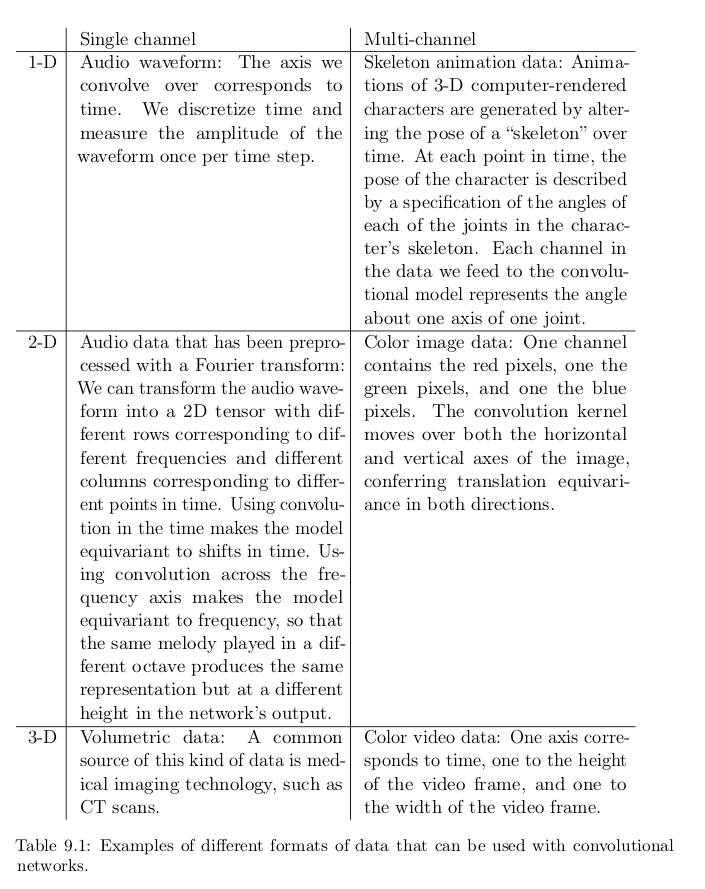
\includegraphics[width=0.7\textwidth]{conv_data.png}
\end{figure}

Convolution for processing variable sized inputs only makes sense for inputs that have variable size because they contain varying amounts of observation of the same kind of thing - different lengths of recordings over time, different widths of observations of space, etc. 

Convolution does \textbf{not} make sense if the input has variable size because it can optionally include different kinds of observations. For example, if we are processing college applications, and our features consist of both grades and standardized test scores, but not every applicant took the standardized test, then it does not make sense to convolve the same weights over both the features corresponding to the grades and the features corresponding to the test scores. 

\section{Efficient Convolution Algorithms}

Convolution is equivalent to converting both the input and the kernel to the frequency domain using a Fourier transform, performing pointwise multiplication of the two signals, and converting back to the time domain using an inverse Fourier transform. For some problem sizes this can be faster than the naive implementation of discrete convolution.

When a $d$-dimensional kernel can be expressed as the outer product of $d$ vectors, one vector per dimension, the kernel is called \textbf{separable}. When the kernel is separable, naive convolution is inefficient. It is equivalent to compose $d$ one dimensional convolutions of each of these vectors. 

The composed approach is significantly faster than performing one $d$-dimensional convolution with their outer product. The kernel also takes fewer parameters to represent as vectors. If the kernel is $w$ elements wide in each dimension, then naive multidimensional convolution requires $O(w^d)$ runtime and parameter storage space, and separable convolution requires $O(w \times d)$ runtime and parameter storage space. 

\section{Random or Unsupervised Features}

There are three basic strategies for obtaining convolutional kernels without supervised training: 

\begin{enumerate}
\item Initialize them randomly
\item design them by hand
\item learn the kernels with an unsupervised criterion
\end{enumerate}

For example \href{http://ai.stanford.edu/~acoates/papers/coatesleeng_aistats_2011.pdf}{Coates et. al} applies k-means clustering to small image patches, then uses each learned centroid as a convolution kernel. 

\begin{quote}
  \textbf{Abstract: } A great deal of research has focused on
  algorithms for learning features from unlabeled data. Indeed, much
  progress has been made on benchmark datasets like NORB and CIFAR by
  employing increasingly complex unsupervised learning algorithms and
  deep models. In this paper, however, we show that several simple
  factors, such as the number of hidden nodes in the model, may be
  more important to achieving high performance than the learning
  algorithm or the depth of the model. Specifically, we will apply
  several offthe-shelf feature learning algorithms (sparse
  auto-encoders, sparse RBMs, K-means clustering, and Gaussian
  mixtures) to CIFAR, NORB, and STL datasets using only singlelayer
  networks. We then present a detailed analysis of the effect of
  changes in the model setup: the receptive field size, number of
  hidden nodes (features), the step-size (“stride”) between extracted
  features, and the effect of whitening. Our results show that large
  numbers of hidden nodes and dense feature extraction are critical to
  achieving high performance—so critical, in fact, that when these
  parameters are pushed to their limits, we achieve state-of-the-art
  performance on both CIFAR-10 and NORB using only a single layer of
  features. More surprisingly, our best performance is based on
  K-means clustering, which is extremely fast, has no hyperparameters
  to tune beyond the model structure itself, and is very easy to
  implement. Despite the simplicity of our system, we achieve accuracy
  beyond all previously published results on the CIFAR-10 and NORB
  datasets (79.6\% and 97.2\% respectively).
\end{quote}

The paper above has the following framework: 

Perform the following steps to learn a feature representation: 

\begin{enumerate}
\item Extract random patches from unlabeled training images
\item Apply a preprocessing stage to the patches
\item Learn a feature mapping using an unsupervised learning algorithm
\item Extract features from equally spaced sub-patches covering the input image
\item Pool features together over regions of the input image to reduce the number of feature values
\item Train a linear classifier to predict the labels given the feature vectors
\end{enumerate}

Where the unsupervised learning algorithms mentioned were the following: 

\begin{enumerate}
\item Sparse Autoencoder 
\item Sparse Restricted Boltzmann Machine
\item K-means Clustering
\item Gaussian Mixtures
\end{enumerate}

Learning the features with an unsupervised criterion allows them to be determined separately from the classifier layer at the top of the architecture. One can then extract the features for the entire training set just once, essentially constructing a new training set for the last layer. Learning the last layer is then typically a convex optimization problem, assuming the last layer is something like logistic regression or an SVM. 

Random filters also often work well. (Jarrett et al. , 2009 ; Saxe et al. , 2011 ; Pinto et al. , 2011 ; Cox and Pinto , 2011 ). Saxe et al. ( 2011 ) showed that layers consisting of convolution following by pooling naturally become frequency selective and translation invariant when assigned random weights. 

They argue that this provides an easy way to choose architectures for conv nets: 
Evaluate select convolutional networks by training only the last layer, then take the best of these architectures and train the entire architecture using a more expensive approach. 

An intermediate approach is to learn the features, but using methods that do not require full forward and backward propagation at every gradient step. We can use greedy layer-wise pretraining to train the first layer in isolation given those features, then extract all features from the first layer only once, then train the second layer in isolation given those features, and so on. The canonical example of greedy layer-wise pretraining of a convolutional model is the convolutional deep belief network: \href{http://www.cnbc.cmu.edu/cns/papers/lee-CDBN.pdf}{Lee et. al (2009)}.

\begin{quote}
  \textbf{Abstract: } There has been much interest in unsupervised
learning of hierarchical generative models such as deep belief
networks. Scaling such models to full-sized, high-dimensional images
remains a difficult problem. To address this problem, we present the
convolutional deep belief network, a hierarchical generative model
which scales to realistic image sizes. This model is
translation-invariant and supports efficient bottom-up and top-down
probabilistic inference. Key to our approach is probabilistic
max-pooling, a novel technique which shrinks the representations of
higher layers in a probabilistically sound way. Our experiments show
that the algorithm learns useful high-level visual features, such as
object parts, from unlabeled images of objects and natural scenes. We
demonstrate excellent performance on several visual recognition tasks
and show that our model can perform hierarchical (bottom-up and
top-down) inference over full-sized images.
\end{quote}

\section{The Neuroscientific Basis for Convolutional Networks}

\href{http://www.cs.toronto.edu/~fritz/absps/langTDNN.pdf}{Lang and Hinton (1988)}

\begin{quote}
  \textbf{Abstract: } A translation-invariant back-propagation network
is described that performs better than a sophisticated continuous
acoustic parameter hidden Markov model on a noisy, lO0-speaker
confusable vocabulary isolated word recognition task. The network's
replicated architecture permits it to extract precise information from
unaligned training patterns selected by a naive segmentation rule.
\end{quote}

Lang and Hunton introduced the use of backpropagation to train \textbf{time-delay neural networks}. TDNNs are one dimensional convolutional networks applied to time series. Following the success of backpropagation based training of TDNNs, 
\href{http://yann.lecun.com/exdb/publis/pdf/lecun-89e.pdf}{LeCun et. al. (1989)} developed the model convolutional network by applying the same training algorithm to 2D convolution applied to images.

\begin{quote}
  \textbf{Abstract: } The ability of learning networks to generalize can be greatly enhanced by providing constraints from the task domain. This paper demonstrates how such constraints can be integrated into a backpropagation network through the architecture of the network. This approach has been successfully applied to the recognition of handwritten zip code digits provided by the U.S. Postal Service. A single network learns the entire recognition operation, going from the normalized image of the character to the final classification.
\end{quote}

\begin{figure}[h]
  \centering
  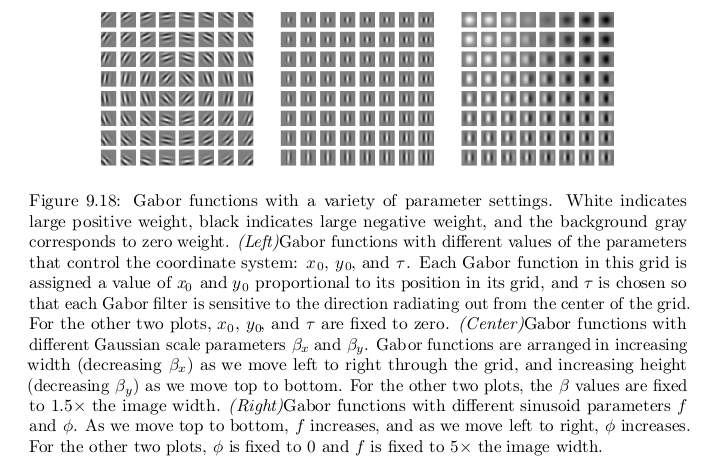
\includegraphics[width=0.7\textwidth]{gabor.png}
\end{figure}


\end{document}
